\documentclass[french]{article}


\usepackage{arxiv}

\usepackage{babel}
\usepackage[utf8]{inputenc} % allow utf-8 input
\usepackage[T1]{fontenc}    % use 8-bit T1 fonts
\usepackage{hyperref}       % hyperlinks
\usepackage{url}            % simple URL typesetting
\usepackage{booktabs}       % professional-quality tables
\usepackage{amsfonts}       % blackboard math symbols
\usepackage{nicefrac}       % compact symbols for 1/2, etc.
\usepackage{microtype}      % microtypography
\usepackage{lipsum}
\usepackage{graphicx}

\title{Intégration de l'outil \\ d'analyse  \emph{Mopsa} dans \emph{Visual Studio Code}   }

\author{
   Gabriel Jeantet \\
   n\textsuperscript{o} étudiant: 28605630 \\
   Parcours STL, Master Informatique\\
   Sorbonne Université\\
   \texttt{gabriel.jeantetpro@gmail.com} \\
    \And
   Mohamed Hernouf \\
   n\textsuperscript{o} étudiant: 3872505 \\
   Parcours STL, Master Informatique\\
   Sorbonne Université\\
   \texttt{hernouf@yandex.ru} \\
   \And
   Claire Bardoux \\
   n\textsuperscript{o} étudiant: 28609617 \\
   Parcours STL, Master Informatique\\
   Sorbonne Université\\
   \texttt{cbardoux26@gmail.com} \\
}

\date{}

\begin{document}
\maketitle

\begin{abstract}
Ce document présente la démarche suivie en cours afin d'effectuer nos recherches pour le projet d'\emph{intégration de l'outil d'analyse Mopsa dans Visual Studio Code}.
\end{abstract}


\section{Introduction}
Des chercheurs du laboratoire \emph{LIP6} developpent un analyseur statique et sémantique de programmes. Cet outil affiche ses résultats et s'utilise à partir d'un terminal. Il génére également un fichier résultat JSON. Visual Studio Code (VSCode) est un éditeur de code extensible. Il permet de s'intégrer facilement à des outils de build, d’analyse de code et de déboguage. Notre but est d'écrire une extension VSCode capable d'integrer Mopsa pour naviguer les résultats de l'analyse. 

Il y a deux aspects principaux: l'exploitation du fichier JSON résultat et l'implantation du \emph{Debug Adapter Protocol}. 
Dans la première partie, nous utilisons la liste et position des erreurs découvertes pour décorer le code sur lequel l'outil a été lancé. Ainsi l'utilisateur voit où il y a des erreurs et peut cliquer sur une variable et retrouver toutes les informations inférées par l’analyseur sur cette variable à ce point. Néanmoins le but est de mettre à jour l'interface au fur et à mesure de l'analyse et d'exécuter l'analyse pas à pas comme dans un débogueur. Pour cela nous devons dévéloper le \emph{Debug Adapter Protocol} dans notre extension VSCode ainsi que dans leur outil.  


\section{Les mots clés retenus}
Nous avons listé les mots utilisés lors de nos recherches bibliographiques et les avons organisées sous forme de carte heuristique.  \\

\begin{figure*}[!b]
  \centering
  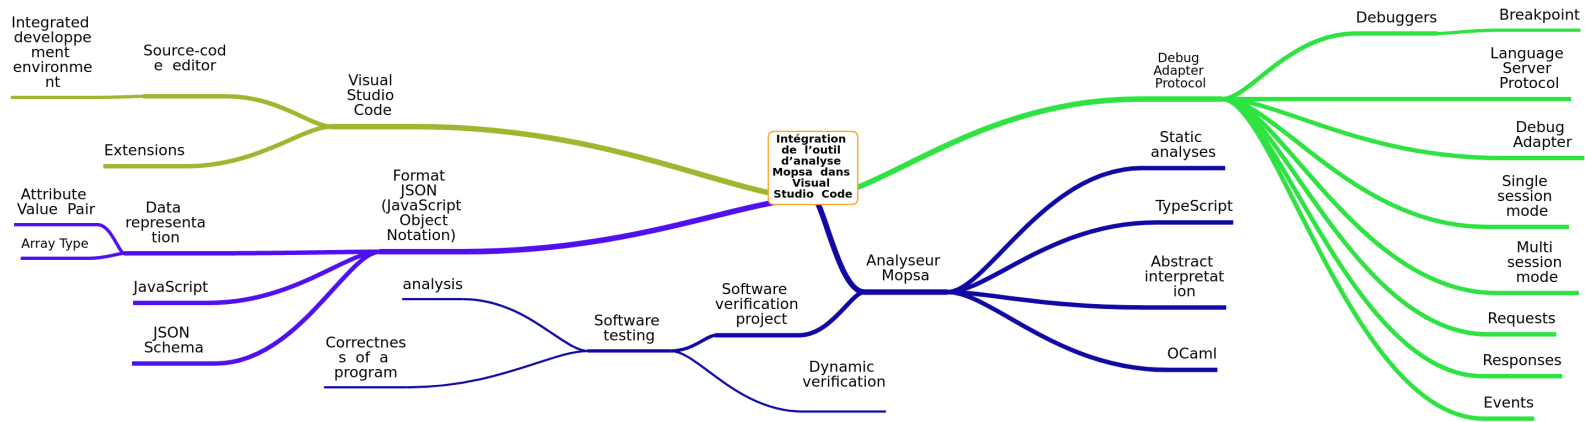
\includegraphics[width=17cm, height=5.80cm]{mindmap.png}
  \caption{Sample figure caption.}
\end{figure*}

Voici la bibliographie : 
\begin{itemize}
\item Debug Adapter Protocol 
\item Analyseur Mopsa \cite{caires_abstract_2019}\cite{rival_static_2016}\cite{delmas_analysis_nodate}\cite{chakraborty_combinations_2020}
\item Format JSON \cite{langdale_parsing_2019},\cite{JavaScriptBook}
\item Visual Studio Code 
\newline
\end{itemize}

 A noter que pour Debug Adapter Protocol et Visual Studio Code les informations sont extraite de sites web officiels mais pas sans être des documents, donc nous ne pouvons les citer dans le bibiliographie. 

\section{Descriptif de la recherche documentaire}
\label{sec:others}
Pour trouver des termes nous avons utilisé \emph{le grand dictionnaire terminologique} et \emph{termsciences}, qui permettent de nous guider sur les termes à privilégier et ceux à eviter. On a également utilisé la page de Wikipedia pour trouver des mots clés réliés ainsi que de l'information en faisant attention à ce qu'elle soit fiable.

Ensuite lorsqu'on avait un mot clé précis on effectuait des recherches d'articles scientifiques dans et les bases de données comme Google Scolar ou Web of Science. Google Scholar trouve beaucoup de résultats mais a très peu de possibilités de tri, tandis que Web of Science c'est tout le contraire. On utilisait également des bases de données spécialisés en informatique tels que ACM ou ArXiv. ArXiv a une publication très rapide et donc des données récentes, néanmoins ils sont si récents que certains documents ont pas eu le temps d'être relu et peuvent être faux.  ACM, propose beaucoup d'outils de tri des articles et contrairement à ArXiv, les articles sont relu avant d'être plubliées, donc plus sûre. 

Nous avons également lu beaucoup de documentation et d'API pour savoir comment écrire notre extension. 

Finalement, grâce au catalogue de la bibliothèque universitaire nous avons pu rechercher les livres qui nous seraient utiles pour apprendre le langage de programmation dans lequel nous developpons. 

\section{Bibliographie produite dans le cadre du projet}

\bibliographystyle{plain}
\bibliography{biblio}


\section{Evaluation des sources}
\begin{tabular}{ |p{1.5cm}||p{6cm}|p{8cm}|  }
 \hline
 \multicolumn{3}{|c|}{Fiabilité des sources} \\
 \hline
 Ressource  & Manière dont on l'a trouvé & Evaluation critique\\
 \hline
 \cite{langdale_parsing_2019}   & Via la base de données arXiv \url{https://arxiv.org/abs/1902.08318} &
 
 \begin{itemize}
\item Date/Fraicheur: L'article a été publié le 22 Février 2019 et jusqu'au deux janvier elle a eu des modification, ce qui prouve de sa fraicheur et véridicité. 
\item Pertinence: Cette information nous a été utile afin de comprendre comment fonctionne le format JSON qui est décrite dans les premières pages. 
\item Provenance: Bien que les articles de arXiv ne sont pas toujours vérifiés, nous pouvons étre sûr que les auteurs sont bien des personnes compétentes dans leurs domaines car nous pouvons retrouver leurs profils et d'autres articles dans le réseau web \emph{ResearchGate}
\item Rigeur du contenu: La qualité de l'information était largement suffisante car nous avons acquis les compétences nécessaires afin d'exploiter sur les fichiers de format JSON. 
\item Objectif: L'information a été écrite afin d'informer d'autres personnes une façon de parser un fichier JSON plus rapidement. 
\newline
\end{itemize} \\

 \cite{caires_abstract_2019}&   Via le site officiel de l'outil Mopsa \url{http://mopsa.lip6.fr/} &  \begin{itemize}
\item Date/Fraicheur:  Avril 2019, c'est la première publication de l'article. 
\item Pertinence: L'information nous a été utile car elle nous a permis de comprendre mieux l'outil pour lequel nous dévélopons une extension. 
\item Provenance: La provenance est vérifié avec sûreté étant donné que les auteurs sont nos tuteurs de projets et les dévéloppeurs de l'outil mopsa. 
\item Rigeur du contenu: Les informations sont tout à fait vérifiable nottament car ils illustrent divers exemples de leur expériences dans leur article. 
\item Objectif: Ce document a pour but d'informer les personnes sur leur outil. 
\newline
\end{itemize}  \\
 \cite{JavaScriptBook} & via le catalogue de la bibliothèque &  \begin{itemize}
\item Date/Fraicheur:  Le livre a été publié en Mars 2011. 
\item Pertinence: Cette information était très importante dans notre projet car nous avions peu de connaissance dans ce langage de programmation.
\item Provenance: L'auteur \emph{David Flanagan} est un développeur et enseignant à \emph{Massachusetts Institute of Technology}, donc la personne est bien qualifié pour parler de ce domaine. 
\item Rigeur du contenu: Plus que suffisante. Les données sont sûres car c'est la sixième edition de ce livre et il est vendu partout dans le monde, et publié par une maison d'édition de renom. 
\item Objectif: C'est un livre à caractère éducatif. 
\newline
\end{itemize}\\
 \hline
\end{tabular}


%\bibliographystyle{unsrt}  
%\bibliography{references}  %%% Remove comment to use the external .bib file (using bibtex).
%%% and comment out the ``thebibliography'' section.


%%% Comment out this section when you \bibliography{references} is enabled.


\end{document}
